\chapter{Post-viva thoughts}
Here are my thoughts in the days that follow my viva. They're a reflection on the areas my examiners require me to address before they will accept my thesis.


\section{Tighten-up the research questions}
The current RQs are too vague to satisfy the examiners. Some need to be more precise \emph{e.g.} rather than use the word quality, identify the particular quality/qualities being covered in the thesis: Reliability/stability in terms of crashes, errors and ANRs.  

\section{Apply the revised RQs throughout the thesis}
Root each chapter to the research questions to help determine and decide what material is relevant in this chapter and how this chapter helps address the research questions without extraneous material.


\section{Be more consistent and more precise}
Use terms consistently, define or reference their meaning in the context of my thesis. I'd done this to a certain extent but clearly not sufficiently to satisfy them. I had used topics, for example, in one of my findings chapters as an alias for themes.

\section{Establishing a clearer chain of evidence of findings}
They believed they had to take-on-trust my findings rather than being able to see examples of how I'd analysed various findings and done so consistently, adequately, and coherently. My external examiner asked why I hadn't provided a reproduction package, AFAIK the OU doesn't encourage such packages so I'll seek advice on how best to make evidence available in my thesis and/or elsewhere. Some ideas include: 
\begin{itemize}
\item Publishing material on my personal blog
\item Publishing articles on medium.com
\item Publishing material on arxiv and adding it to ORO
\end{itemize}

\begin{figure}
    \centering
    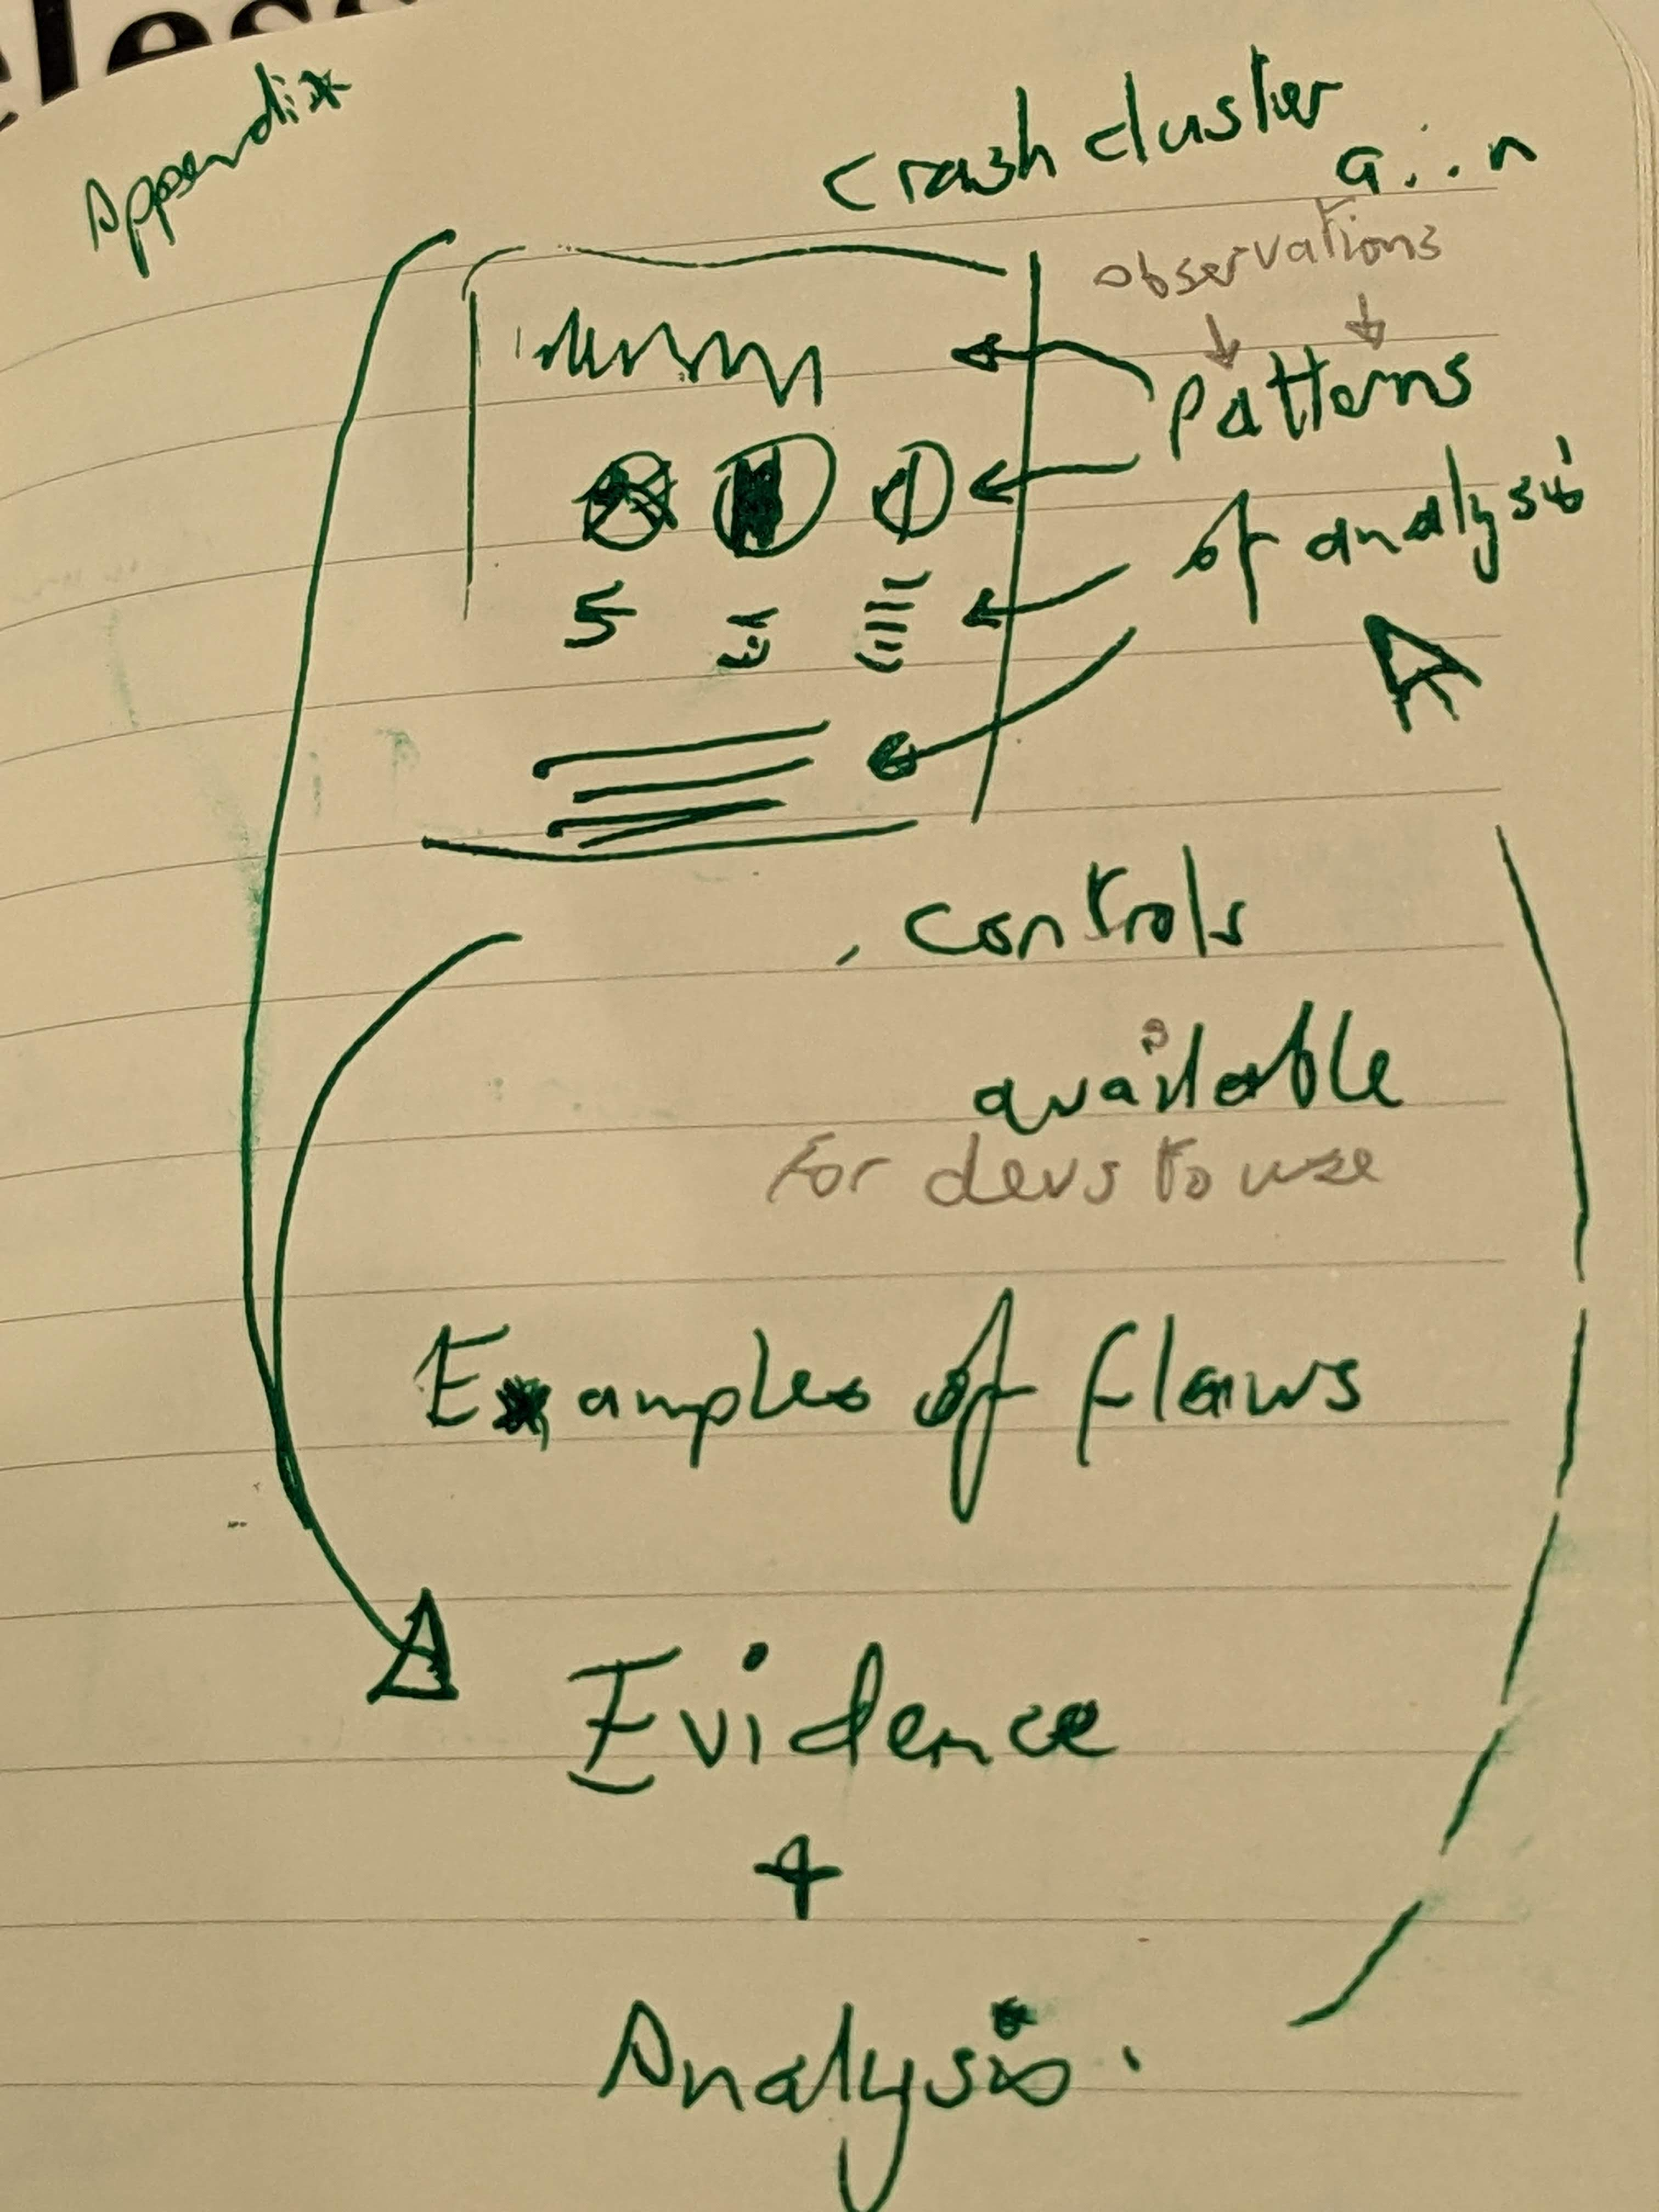
\includegraphics{images/rough-sketches/evidence_and_analysis_cycle.jpeg}
    \caption{Evidence and analysis feedback cycle}
    \label{fig:evidence_and_analysis_cycle}
\end{figure}
Screenshots (discussed in the next section) might well be a useful and succinct source of evidence to demonstrate to my readers (including my examiners). Techniques, such as contact sheets \sidecite[][p.74]{harty2009_practical_guide_to_testing_wireless_smartphone_applications}, combined into composite images to reduce the \LaTeX compilation overhead, might be worth adding to my thesis. 


\section{Evidence and analysis feedback cycle}
Figure \ref{fig:evidence_and_analysis_cycle} represents a screenshot for a crash cluster report, provided by, and in, Android Vitals. The developer may have various controls available in the UI that would enable them to vary the information presented on screen. They may also be able to capture a screenshot of part, or all, of the report and/or extract content from the report.

The screenshot is a source of evidence; similarly any content extracted and preserved from the report may be another source of evidence. which needs to be analysed to provide findings. Note: the findings can potentially be grouped into themes, as discussed in the next section. 

The feedback cycle helps from a research perspective: the patterns of analysis (and a clearer version of Figure \ref{fig:evidence_and_analysis_cycle}) should be incorporated into my thesis - possibly in the Methodology chapter.


\section{Thematic Analysis Revisited}
My external examiner asked me to use an existing approach to thematic analysis that they would recognise, rather than one I invented (\emph{i.e.} don't reinvent the wheel). After pondering the sanity of this advice - given I'd already performed my own thematic analysis - I think I now have a better idea how her advice might apply and how I can at least do due diligence on her proposal. 

Pre-viva the themes were inspired by grounded theory \emph{i.e.} they emerged as part of reviewing the many and various findings I'd gathered over the years of the research. They were then refined with the active participation of my supervisors. I then started to identify higher-level themes and initially had quite a few of these. Again these were refined and also combined to reduce the set of higher-level themes in order to set the context for each of the findings chapters.

Post-viva I get the impression that what my external examiner wants me to do is essentially start again from my collection of findings. This time, I'm to select and apply at least one of the methods to perform thematic analysis that has been established through the `literature' \emph{e.g.} selected from a oft-cited recognised academic text book. I'm then to use that methodology on my set(s) of findings and see what I end up with in terms of the lower-level (L1) themes. I'd then use the same method (at least in the first instance) to identify higher-level groupings of the lower-level themes. I'd do some analysis of both the lower- and the higher- level themes. I'd then restructure my findings chapters using these themes.

Figure \ref{fig:thematic-analysis-revisited-sketch} was my first attempt at realising what I've been asked to do.\sidenote{Drawn on \nth{2} December 2022}

I'd keep doing so until we reach a point of vanishing returns or if I'm able to demonstrate the existing, recognised, methods are inadequate for my research. In the process I'd learn how to apply the discipline of subjecting my research to a pre-existing methodology and approach.

\begin{figure}
    \centering
    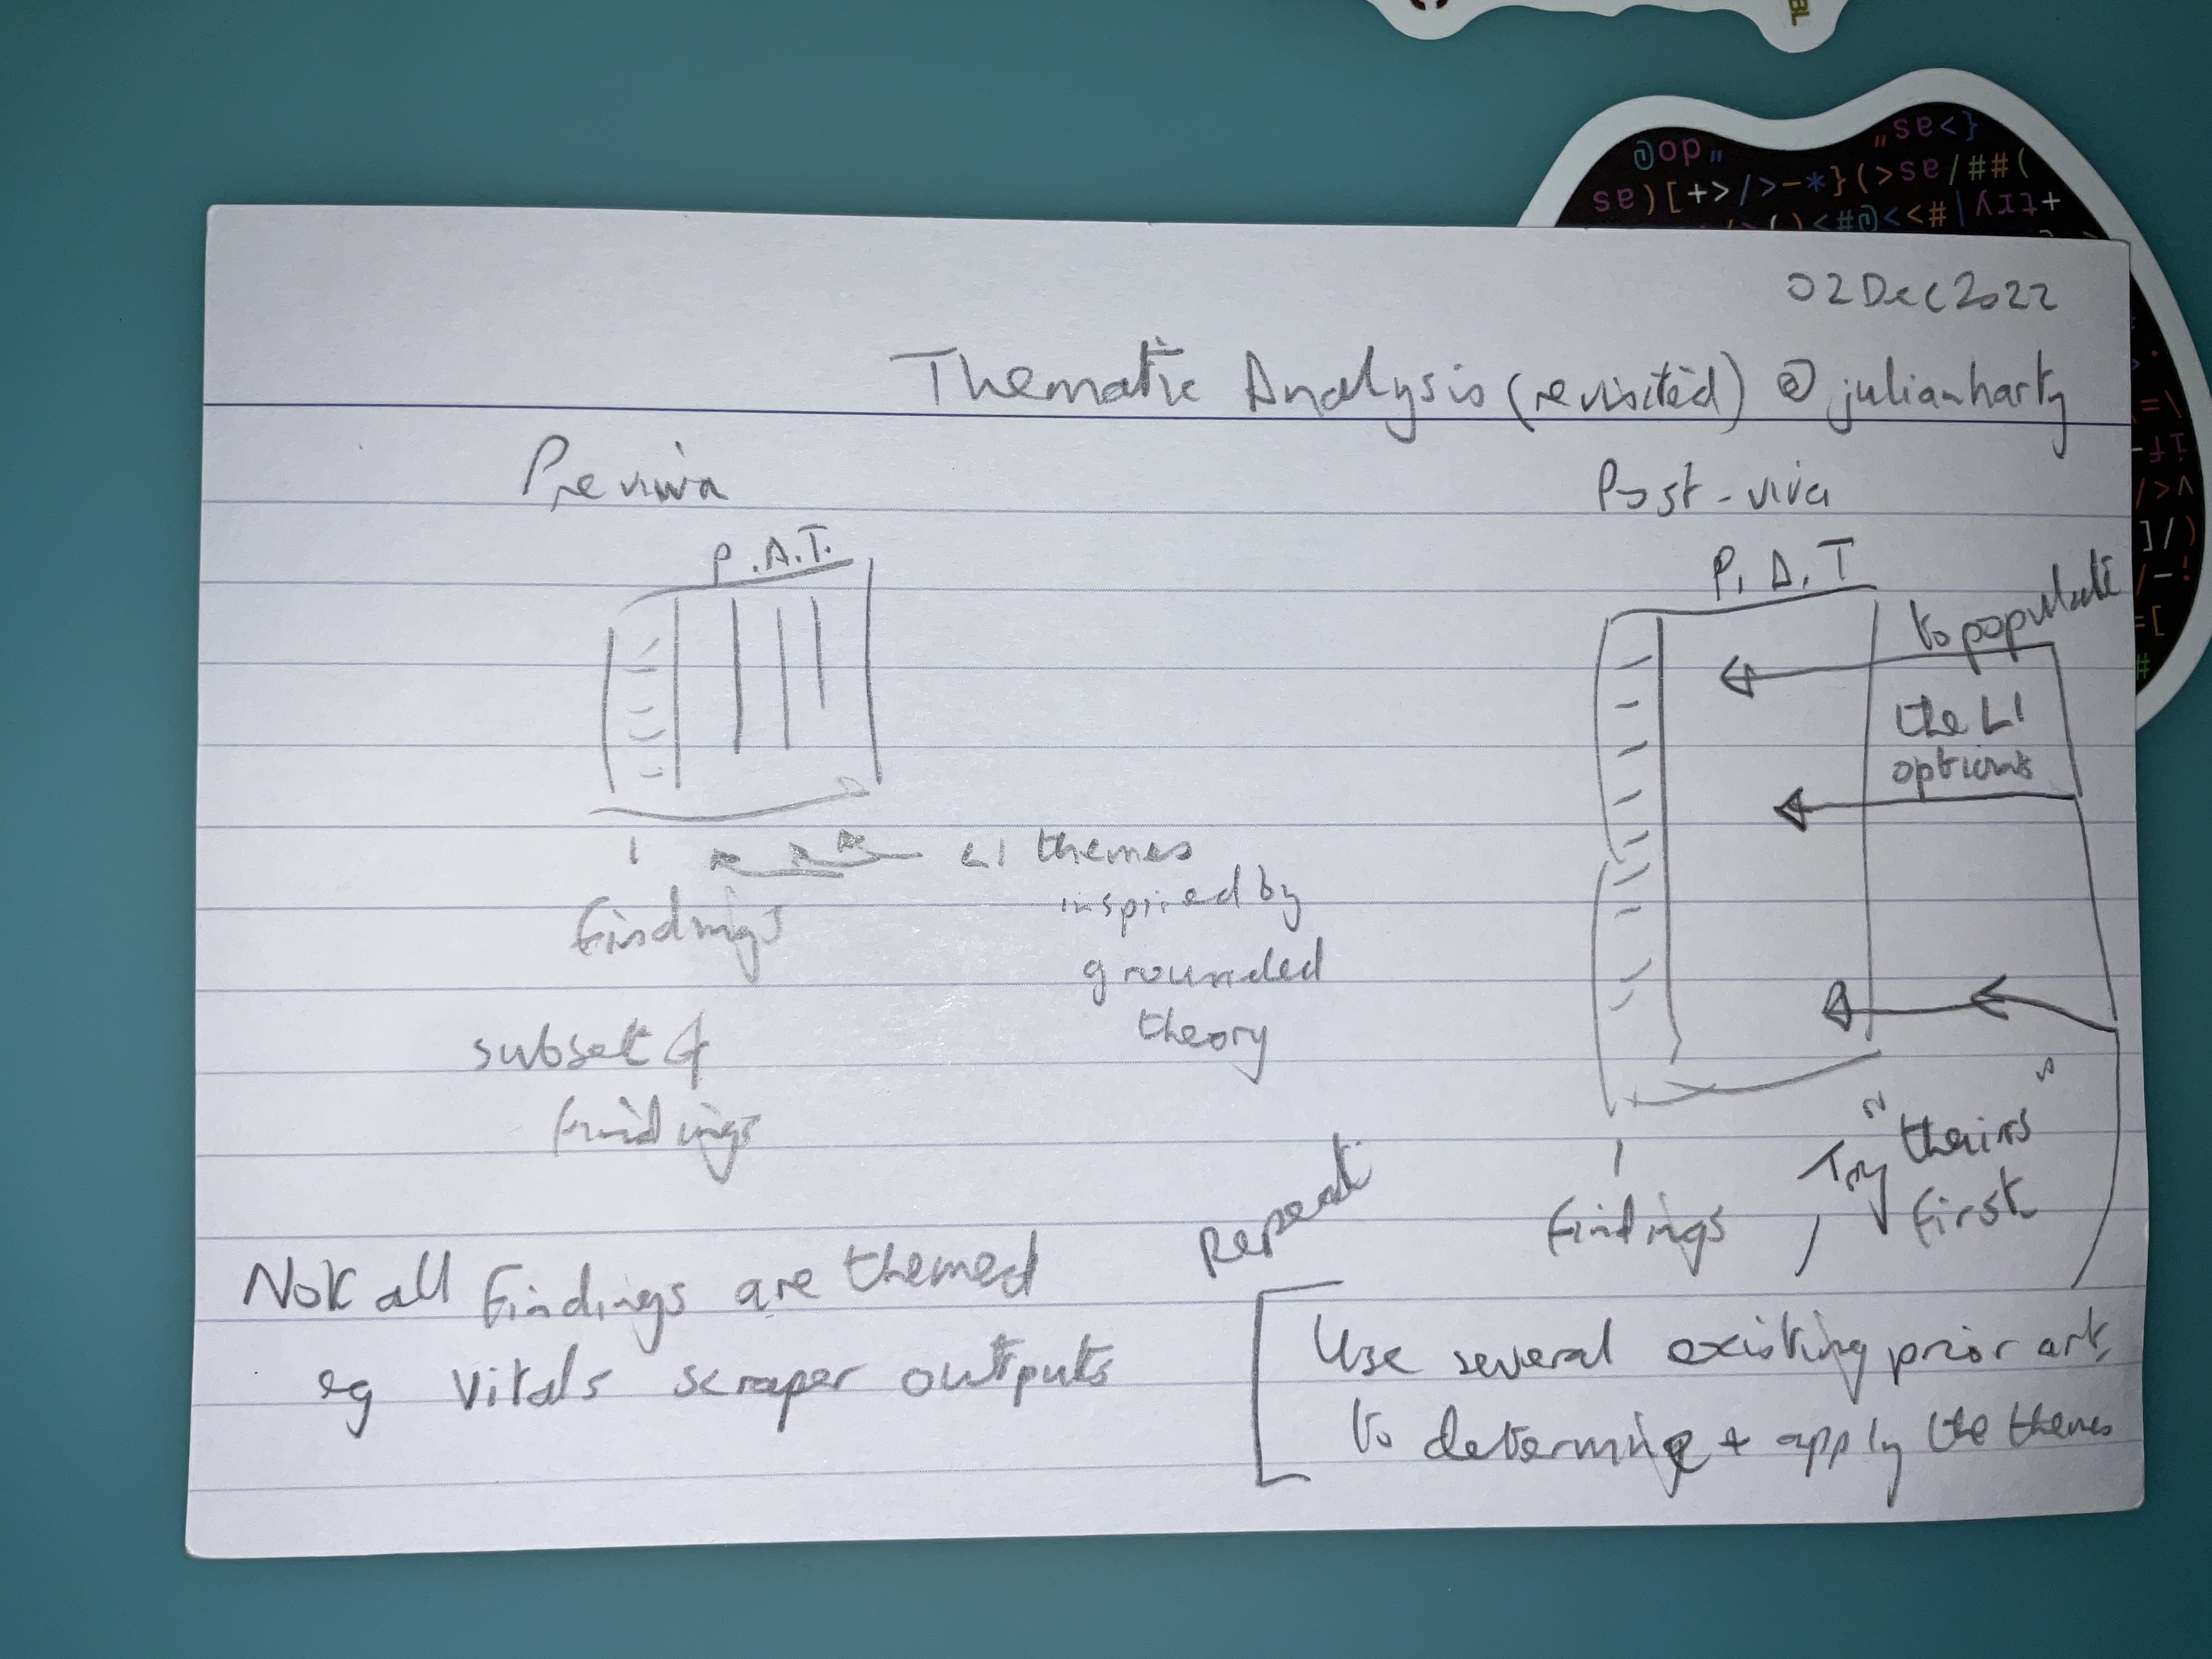
\includegraphics{images/rough-sketches/thematic-analysis-revisited-sketch.jpeg}
    \caption{Thematic Analysis revisited}
    \label{fig:thematic-analysis-revisited-sketch}
\end{figure}


\subsection{Flick \emph{et al}}
In chapter 5.11 of \sidecite[][pp. 259-265]{flick2004_triangulation_in_qualitative_research} Rosenthal and Fischer-Rosenthal cover the analysis of narrative-biographical interviews. My research includes various interviews of members of development teams so this material is potentially relevant, and potentially useful.
However, their focus is in the domain of social sciences, life histories, and life-stories. They discuss life-as-narrated vs life-as-lived. They do not provide detail of how they perform their thematic field analysis. So their work is not particularly actionable in terms of my research.
